\documentclass[aps,twocolumn,secnumarabic,balancelastpage,amsmath,amssymb,nofootinbib]{revtex4}
% \documentclass[aps,twocolumn,secnumarabic,balancelastpage,amsmath,amssymb,nofootinbib]{revtex4}

% Documentclass Options

% nobalancelastpage doesn't attempt to equalize the lengths of the two columns
% on the last page as might be desired in a journal where articles follow one
% another closely
% amsmath and amssymb are necessary for the subequations environment among
% others secnumarabic identifies sections by number to aid electronic review
% and commentary. nofootinbib forces footnotes to occur on the page where they
% are first referenced and not in the bibliography

% \usepackage{lgrind}        % convert program listings to a form includable in a LaTeX document
\usepackage{chapterbib}    % allows a bibliography for each chapter (each labguide has it's own)
\usepackage{color}         % produces boxes or entire pages with colored backgrounds
\usepackage{graphics}      % standard graphics specifications
\usepackage[pdftex]{graphicx}      % alternative graphics specifications
\usepackage{longtable}     % helps with long table options
\usepackage{epsf}          % old package handles encapsulated post script issues
\usepackage{bm}            % special 'bold-math' package
\usepackage{tikz}
\usepackage{asymptote}     % For typesetting of mathematical illustrations
\usepackage{subfigure}

% \usepackage{thumbpdf}

\usepackage[colorlinks=true]{hyperref}  % this package should be added after all others
% use as follows: \url{http://web.mit.edu/8.13}
\newcommand{\drelectron}[1]{\node at #1 [circle, draw, inner sep=0pt, minimum size=1pt] {\_}}
\newcommand{\ud}{\mathrm{d}}
\newcommand{\ue}{\mathrm{e}}
\newcommand{\ui}{\mathrm{i}}
\newcommand{\res}{\mathrm{Res}}
\newcommand{\Tr}{\mathrm{Tr}}
\newcommand{\dsum}{\displaystyle\sum}
\newcommand{\dprod}{\displaystyle\prod}
\newcommand{\dlim}{\displaystyle\lim}
\newcommand{\dint}{\displaystyle\int}
\newcommand{\fsno}[1]{{\!\not\!{#1}}}
\newcommand{\eqar}[1]
{
  \begin{align*}
    #1
  \end{align*}
}
\newcommand{\texp}[2]{\ensuremath{{#1}\times10^{#2}}}
\newcommand{\dexp}[2]{\ensuremath{{#1}\cdot10^{#2}}}
\newcommand{\eval}[2]{{\left.{#1}\right|_{#2}}}
\newcommand{\paren}[1]{{\left({#1}\right)}}
\newcommand{\lparen}[1]{{\left({#1}\right.}}
\newcommand{\rparen}[1]{{\left.{#1}\right)}}
\newcommand{\abs}[1]{{\left|{#1}\right|}}
\newcommand{\sqr}[1]{{\left[{#1}\right]}}
\newcommand{\crly}[1]{{\left\{{#1}\right\}}}
\newcommand{\angl}[1]{{\left\langle{#1}\right\rangle}}
\newcommand{\tpdiff}[4][{}]{{\paren{\frac{\partial^{#1} {#2}}{\partial {#3}{}^{#1}}}_{#4}}}
\newcommand{\tpsdiff}[4][{}]{{\paren{\frac{\partial^{#1}}{\partial {#3}{}^{#1}}{#2}}_{#4}}}
\newcommand{\pdiff}[3][{}]{{\frac{\partial^{#1} {#2}}{\partial {#3}{}^{#1}}}}
\newcommand{\diff}[3][{}]{{\frac{\ud^{#1} {#2}}{\ud {#3}{}^{#1}}}}
\newcommand{\psdiff}[3][{}]{{\frac{\partial^{#1}}{\partial {#3}{}^{#1}} {#2}}}
\newcommand{\sdiff}[3][{}]{{\frac{\ud^{#1}}{\ud {#3}{}^{#1}} {#2}}}
\newcommand{\tpddiff}[4][{}]{{\left(\dfrac{\partial^{#1} {#2}}{\partial {#3}{}^{#1}}\right)_{#4}}}
\newcommand{\tpsddiff}[4][{}]{{\paren{\dfrac{\partial^{#1}}{\partial {#3}{}^{#1}}{#2}}_{#4}}}
\newcommand{\pddiff}[3][{}]{{\dfrac{\partial^{#1} {#2}}{\partial {#3}{}^{#1}}}}
\newcommand{\ddiff}[3][{}]{{\dfrac{\ud^{#1} {#2}}{\ud {#3}{}^{#1}}}}
\newcommand{\psddiff}[3][{}]{{\frac{\partial^{#1}}{\partial{}^{#1} {#3}} {#2}}}
\newcommand{\sddiff}[3][{}]{{\frac{\ud^{#1}}{\ud {#3}{}^{#1}} {#2}}}

\begin{document}
\tikzstyle{every picture}+=[remember picture]
\title{Optical Pumping of Rubidium Atoms in the Magnetic Field.}
\author{Yichao Yu}
\email{yuyichao@mit.edu}
\homepage{http://yyc-arch.org/}
\date{\today}
\affiliation{MIT Department of Physics}

\begin{abstract}
  The optical pumping is a technique that uses light to obtain non-thermal energy level distribution. It is important for atomic physics for state preparation and maintaining and is used in some standard laser cooling and trapping techniques. In this experiment, we studied the optical pumping between Zeeman levels in a magnetic field of rubidium atoms causing by a polarized light. We were able to measure some steady state properties like Landr\'e $g$-factors, abundance and ambient magnetic field as well as observe the transient state and measure the pumping rate and Rabi frequency.
\end{abstract}

\maketitle
%%%%%%%%%%%%%%%%%%%%%%%%%%%%%%%%%%%%%%%%%%%%%%%%%%%%%%%%%%%%%%%%%%
\section*{Introduction}
At thermal equilibrium, the population of energy levels of atoms is given by the Maxwell-Boltzmann distribution,
\[ \frac{n_1}{n_2}=\exp\paren{\frac{E_2-E_1}{k_BT}} \]

In the case of rubidium atoms at around room temperature ($300K$), the hyper-fine splitting (around $20\mu eV$) and the Zeeman splitting in a weak ($<1Gs$) magnetic field (around $1neV$) is several orders of magnitude smaller than the thermal energy scale ($k_BT\approx20meV$) and therefore have equal occupation numbers in the thermal equilibrium. Optical pumping, however, can be used to break this equilibrium and ``pump'' almost all the atoms into a single Zeeman level using a circularly polarized light. The technique is very important and useful in atomic physics experiment either to prepare a starting state or to keep atoms in a certain state. It is also used in some standard laser cooling and trapping techniques like Zeeman slower and magnetic trap.

In our experiment, we studied the optical pumping of both ${}^{85}Rb$ and ${}^{87}Rb$ atoms using a rubidium lamp and a rubidium vapor cell at around $320K$. By changing the magnetic field and applying a radio frequency signal, we were able to measure the condition when the pumping happens or is destroyed as well as the transient state of the process.

\section{Theory.}
\subsection{Optical pumping between Zeeman levels using circularly polarized light.}
\begin{figure}
  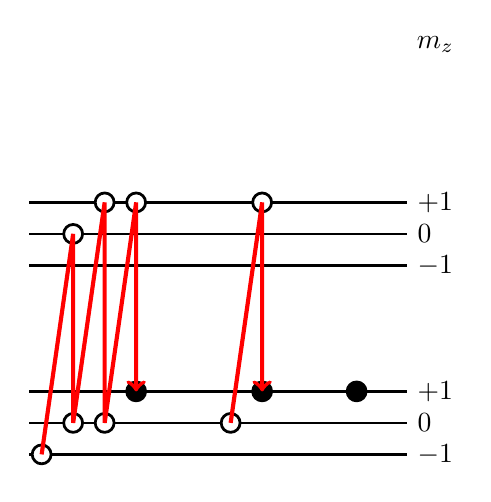
\begin{tikzpicture}[scale=.8]
    \path (6, 6) node[right] {$m_z$};
    \draw[line width=1] (0, 3.5) -- (6, 3.5) node[right] {$+1$};
    \draw[line width=1] (0, 3) -- (6, 3) node[right] {$0$};
    \draw[line width=1] (0, 2.5) -- (6, 2.5) node[right] {$-1$};

    \draw[line width=1] (0, 0.5) -- (6, 0.5) node[right] {$+1$};
    \draw[line width=1] (0, 0) -- (6, 0) node[right] {$0$};
    \draw[line width=1] (0, -0.5) -- (6, -0.5) node[right] {$-1$};

    \draw[line width=1, fill=white] (0.2, -0.5) circle (0.15);
    \draw[line width=1, fill=white] (0.7, 3) circle (0.15);
    \draw[line width=1, fill=white] (0.7, 0) circle (0.15);
    \draw[line width=1, fill=white] (1.2, 3.5) circle (0.15);
    \draw[line width=1, fill=white] (1.2, 0) circle (0.15);
    \draw[line width=1, fill=white] (1.7, 3.5) circle (0.15);
    \draw[line width=1, fill=black] (1.7, 0.5) circle (0.15);

    \draw[line width=1, fill=white] (3.2, 0) circle (0.15);
    \draw[line width=1, fill=white] (3.7, 3.5) circle (0.15);
    \draw[line width=1, fill=black] (3.7, 0.5) circle (0.15);

    \draw[line width=1, fill=black] (5.2, 0.5) circle (0.15);

    \draw[red, ->, line width=1.5] (0.2, -0.5) -- (0.7, 3) -- (0.7, 0)
    -- (1.2, 3.5) -- (1.2, 0) -- (1.7, 3.5) -- (1.7, 0.5);
    \draw[red, ->, line width=1.5] (3.2, 0) -- (3.7, 3.5) -- (3.7, 0.5);
  \end{tikzpicture}
  \caption{Zeeman levels pumping process by circularly polarized light.}
  \label{pumping}
\end{figure}
When placing atoms in a magnetic field, the energy levels with the same total angular momentum $F > 0$ but different angular momentum projection in the field direction $m_F$ will split into $2F + 1$ equally spacing Zeeman levels with a separation given by,
\[ \Delta E=g_F\mu_BB \]
where $\mu_B$ is the Bohr magneton and $g_F$ is the Landr\'e $g$-factor. In the approximation of electron spin $g$-factor $g_e=2$ and ignoring the nuclear magnetic momentum (which is $3$ orders of magnitude smaller), $g_F$ is given by,
\eqar{
  g_J=&\frac{3}{2}+\frac{S(S+1)-L(L+1)}{2J(J+1)}\\
  g_F=&g_J\frac{F(F+1)-I(I+1)+J(J+1)}{2F(F+1)}
}
where $S=\dfrac12$ is the electron spin, $L=0$ and $J=\dfrac12$ for ground of $Rb$ atoms are the orbit angular momentum and spin-orbit coupled angular momentum and $I$ and $F$ are the nuclear and total angular momentum. For the states we are interested in this experiment, $I=\dfrac52$ and $F=3$ for ${}^{85}Rb$ atoms and $I=\dfrac32$ and $F=2$ for ${}^{87}Rb$ atoms.

The interaction between a incident photon and the Zeeman levels is sensitive to the light polarization. For a left handed circularly polarized light along the field direction, the transition when absorbing a photon must have $\Delta m_F=+1$ ($-1$ for right handed light). The spontaneous emission shortly after this can have $\Delta m_F=0, \pm1$. Therefore, using a circularly polarized, we can on average increase $m_F$ by $+1$ (or $-1$ for opposite polarization) for each transition cycle. After several transition as shown in figure \ref{pumping}, (almost) all atoms will end up in the state with largest $m_F$ ($F=3$ $m_F=3$ for ${}^{85}Rb$ atoms and $F=2$ $m_F=2$ for ${}^{87}Rb$ atoms.). Since the excited state of the $D_1$ transition we are using in the experiment $5P_{1/2}$ has the same maximum $m_F$ as the ground state, the result of the pumping is a dark state in which the atoms are not able to absorb the pump light because there is not a state with higher $m_F$ for the atom to go and the absorption of the pump light will change as a result.

\subsection{Depolarization using radio frequency.}
In order to measure the pumping more accurately, instead of directly measuring the absolute absorption of the pumping light, which can change because of ambient light as well as the fluctuation in the light source, we can measure the change of absorption when the dark state is forming or being destroyed. This can be done either by changing the magnetic field non-adiabatically or by applying a radio frequency field.
Since different Zeeman levels have different magnetic momentum, a radio frequency field in resonance with the Zeeman splitting is able to cause a magnetic dipole transition with probability,
\[ P\propto\abs{\Delta \mu B}^2\propto\abs{g_F\mu B}^2 \]
By either changing the magnetic field or the radio frequency and looking for when the resonance happens, we will be able to measure the relation between Zeeman splitting and the magnetic field.

\subsection{Transient Effects}
Besides the steady property of the dark state, there are also some transient effect we can study in the experiment.
\subsubsection{Pumping rate}
The pumping process is a decay to the final state with the time constant(s) of the decay determined by the pumping rate and various spontaneous transition (causing by e.g. atoms collision). By measuring the decay time at different light intensity, we can study the relation between pumping light intensity and the pumping rate.

\subsubsection{Rabi Oscillation}
When driven by the radio frequency field, the atom will undergo a Rabi oscillation before decaying to the stable point. The frequency of this oscillation (Rabi frequency) is related to the coupling between the field and the states. Within the precision of this experiment we are able to measure the Rabi frequency when turning on the radio frequency field as well as their proportionality to the Landr\'e $g$-factor of the two isotopes.

\section{Apparatus}
\begin{figure}
  \begin{tikzpicture}[scale=.8]
    \draw[line width=.2, dashed, red] (0, 0) -- (3, 1) -- (7, 1) -- (9, 0);
    \draw[line width=.2, dashed, red] (0, 0) -- (3, -1) -- (7, -1) -- (9, 0);
    \draw[line width=.2, dashed, red] (0, 0) -- (3, 0) -- (7, 0) -- (9, 0);

    \draw (0, 0) circle (.2);
    \path (0, -.3) node[below] {$Rb$ Lamp};

    \draw[line width=1.2] (1, -1) -- (1, 1) node[above] {$P$};
    \draw[line width=1.2] (2, -1) -- (2, 1) node[above] {$\dfrac{\lambda}{4}$};
    \draw[line width=1.2, <->] (3, -1) -- (3, 1);

    \draw (5, 0) circle (.6) node {$Rb$};

    \draw (5, .7) ellipse (.7 and .05);
    \draw (5, -.7) ellipse (.7 and .05);
    \path (5, -.75) node[below] {rf};

    \draw[line width=2, brown] (4, 0) ellipse (.3 and 2);
    \draw[line width=2, brown] (6, 0) ellipse (.3 and 2);
    \path (5, 1.7) node[above] {$B$};

    \draw[line width=1.2, <->] (7, -1) -- (7, 1);
    \draw (9, 0) circle (.2);
    \path (9, -.3) node[below] {Detector};
  \end{tikzpicture}
  \caption{Experimental apparatus. Only one of the three pairs of Helmholtz coils is drawn for simplicity.}
  \label{apparatus}
\end{figure}

Figure \ref{apparatus} shows the basic setup of this experiment. The light from a rubidium lamp is first turned into circular polarization using a circular polarizer consists of a linear polarizer and a quarter wave plate and then collimated using a lens. The light after absorbed by a rubidium vapor cell is then focused again by a lens onto a photo detector to measure the power. Three pairs of Helmholtz coils (with only one shown on the sketch) are used to control the magnetic field. There are also smaller coils to apply the radio frequency field used to depolarize the pumped atoms.

\section{Measurements and Results}
\subsection{Measurement of Landr\'e $g$-factors by scanning magnetic field at different radio frequency.}
\begin{figure}
  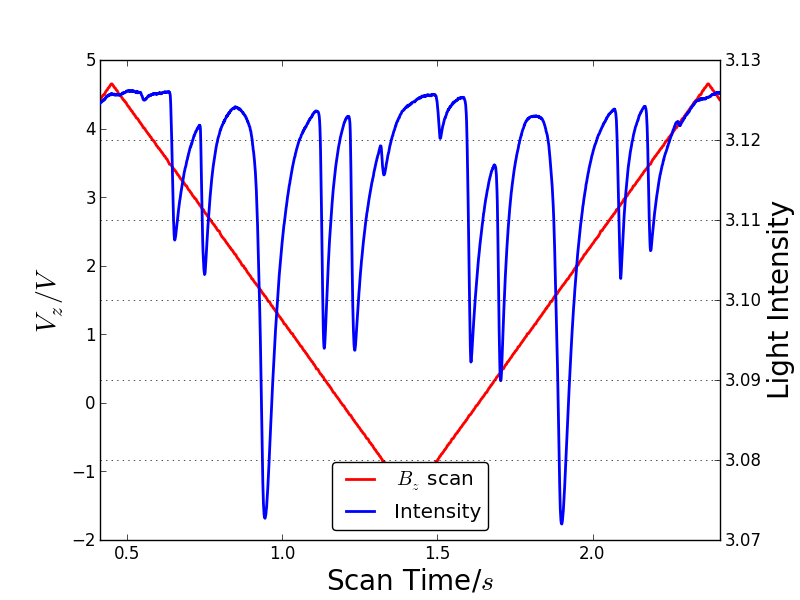
\includegraphics[width=8cm]{../bscan_nf/03-15-bscan_nf_rf1.png}
  \caption{Light intensity when scanning magnetic field with radio frequency field at $100kHz$.}
  \label{bscan_raw}
\end{figure}
\begin{table}
  \begin{tabular}{|c|c|c|}
    \hline
    Isotope&Measured&Expected\\\hline
    ${}^{85}Rb$&$0.498(19)$&$0.500$\\\hline
    ${}^{87}Rb$&$0.331(13)$&$0.333$\\\hline
  \end{tabular}
  \caption{Landr\'e $g$-factors of the two isotopes with theoretical values.}
  \label{g_factor_res}
\end{table}
By sweeping the magnetic field in one direction, we can find the field for the radio frequency to be resonance with the Zeeman splitting. Figure \ref{bscan_raw} shows the light intensity as well as the voltage to create the bias field in $z$ direction of one scan with a $100kHz$ radio frequency field. The larger two dips in the light intensity correspond to the magnetic field to be zero when the Zeeman levels are degenerate and no pumping can happen. The eight smaller dips are the resonance dips when the radio frequency is in resonance with the Zeeman splitting of the two isotopes and increases the absorption and the even smaller dips in the intensity are because of the higher order resonance in the radio frequency field which will resonance with the Zeeman levels at a stronger field.

After finding the position of the dips in the intensity and calculating the energy gap as well as the corresponding field from the radio frequency and the voltage we apply on the coil, we can fit them with a straight line and calculate the Landr\'e $g$-factors for the two isotopes. Table \ref{g_factor_res} shows the results from our data, which agree with the theoretical values within less than one $\sigma$.

\subsection{Measurement of ambient magnetic field and natural abundance by scanning radio frequency at different magnetic field.}
\begin{figure}
  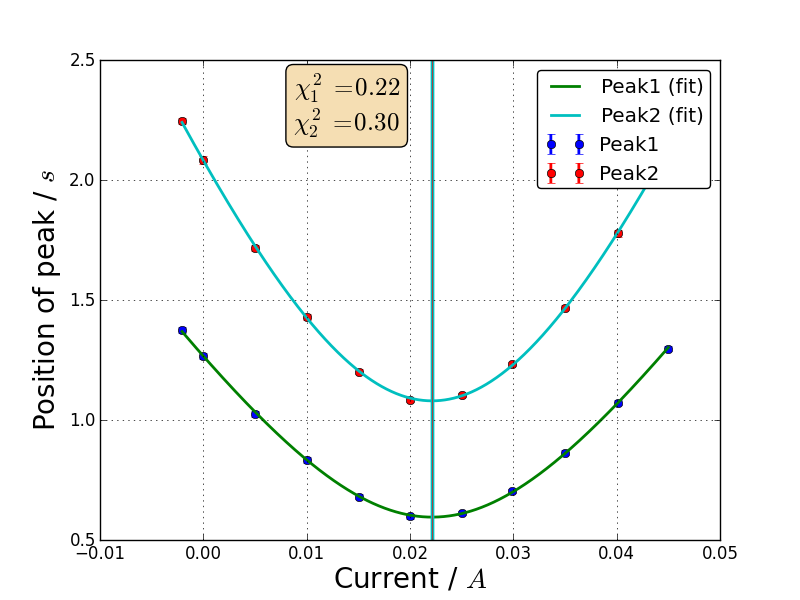
\includegraphics[width=8cm]{../rfscan_nf/rfscan_y_fit.png}
  \caption{Peak positions at different $y$ current}
  \label{rfscan_fit}
\end{figure}
\begin{table}
  \begin{tabular}{|c|c|}
    \hline
    $B_x/mGs$&$361(10)$\\\hline
    $B_y/mGs$&$72.2(1.6)$\\\hline
    $B_z/mGs$&$191.6(5.2)$\\\hline
  \end{tabular}
  \caption{Ambient magnetic field in each directions. The $x$ direction is pointing downward whereas the other two axes are determined by the orientation of the equipment but not aligned with any geometry axis.}
  \label{ambient_field_res}
\end{table}
\begin{table}
  \begin{tabular}{|c|c|c|}
    \hline
    Isotope&Measured&Expected\\\hline
    ${}^{85}Rb$&$72.0(2.2)\%$&$72.168\%$\\\hline
    ${}^{87}Rb$&$28.0(2.2)\%$&$27.835\%$\\\hline
  \end{tabular}
  \caption{Abundance of different $Rb$ isotopes with acceptable values.}
  \label{abundance_res}
\end{table}
By sweeping the radio frequency with different bias magnetic field in each directions, we can find the resonance frequency for each field configuration. By fitting the resonance position with the bias field using a hyperbolic function with taken into account the field in all directions, we can find the minimum resonance frequency for each direction which is the point when the field in this direction is cancelled by the bias field. We also calculated the abundance of the isotopes using this measurement since it appears to be the cleanest measurement. Since the depth of the dips are proportional to the number of atoms the radio frequency signal is able to pull down from the dark state, the depth is not only depending on the abundance of different isotopes but is also proportional to the transition probability causing by the radio frequency field which is proportional to $g_F^2$.

Figure \ref{rfscan_fit} shows the result of this measurement for both isotopes when changing the field in $y$ direction. The resonance point is shown as the position of the dips within the linear frequency scan. The result of this ambient field measurement is shown in table \ref{ambient_field_res}. The total field appears to be smaller than the expected earth field and possible reason that causes this may be the field from other equipment in the lab. Using the amplitude of the intensity dips and the $g_F$ factors we got from previous measurement the result of the abundance of the two isotopes are shown in table \ref{abundance_res}, which are also within one $\sigma$ with the expected natural abundance.

\subsection{Measurement of pumping rate by switching magnetic field on and off at different pumping light intensity.}
\begin{figure}
  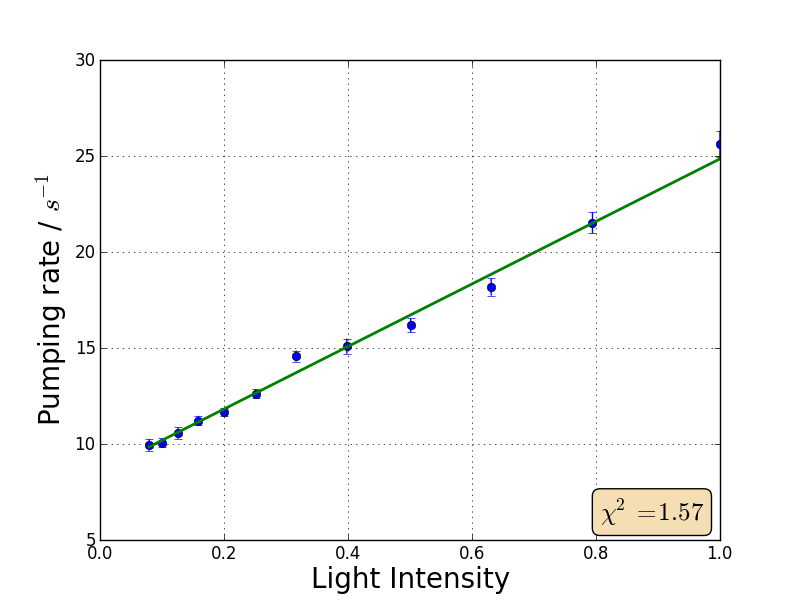
\includegraphics[width=8cm]{../bswitch_nf/03-19-bswitch_nf_od_tau.png}
  \caption{Pumping rate at different light intensity.}
  \label{rate_fit}
\end{figure}
When changing the magnetic field non-adiabatically (e.g. suddenly change the direction of the field in one axis) the already pumped atoms will not be able to follow the new pumped state and will be pumped after each time the field changes. By switching the magnetic field back and forth in the $z$ direction without any radio frequency field, we are able to measure the light intensity during each pumping process. By fitting a exponential decay to the intensity, the inverse of the decay time constant will give us a measure of the pumping rate.

The result of this measurement at different light intensity is shown in plot \ref{rate_fit}. By fitting a straight line to the data, we have found that the pumping rate is linear to the intensity of the pumping light as one would expected intuitively.

\subsection{Measurement of Rabi Oscillation by switching radio frequency on and off at different magnetic field and frequency.}
\begin{figure}
  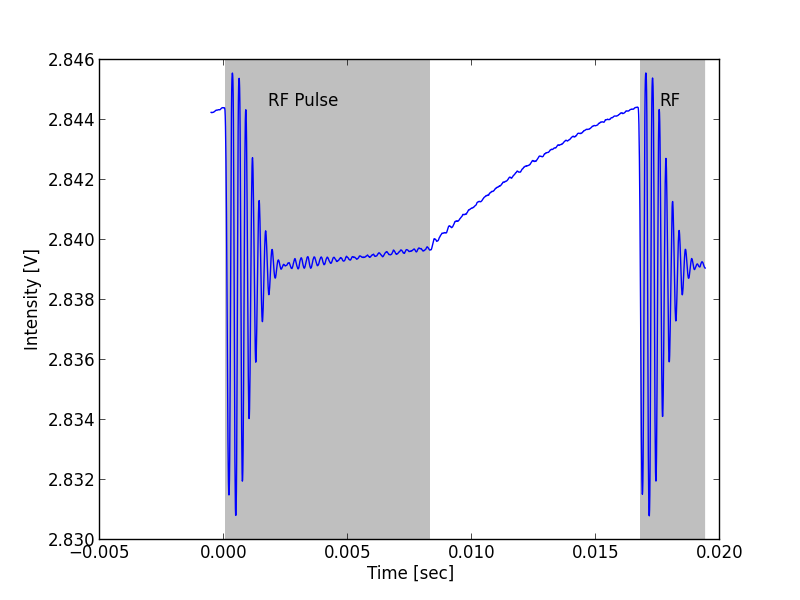
\includegraphics[width=8cm]{../analysis/graphics/rabi_overview.png}
  \caption{Rabi oscillation observed when applying radio frequency. A short pumping time is used in order to see the very short Rabi oscillation period and the pumping period at the same time.}
  \label{rabi_overview}
\end{figure}
\begin{figure}
  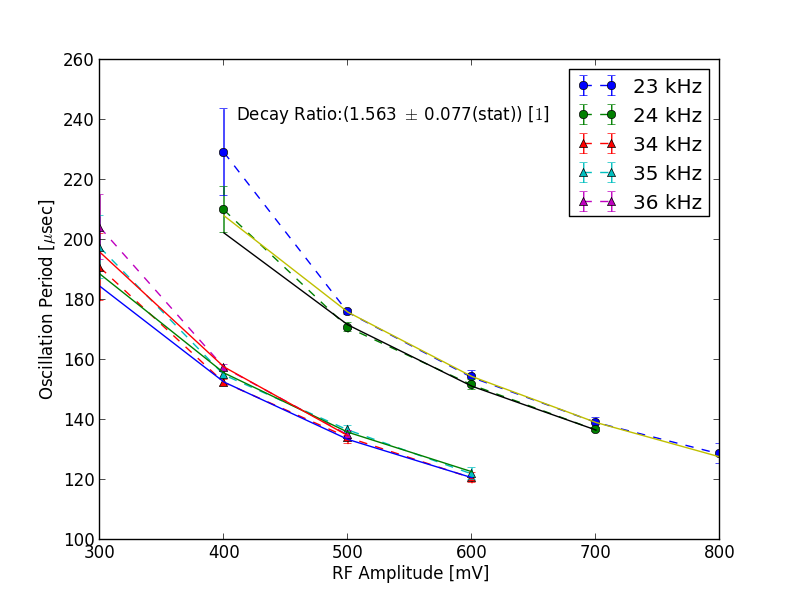
\includegraphics[width=8cm]{../analysis/graphics/rabi_fit.png}
  \caption{Relation between Rabi frequency and the amplitude of the radio frequency signal.}
  \label{rabi_fit}
\end{figure}

By turning the radio frequency field on and off and zooming into the region right after the radio frequency field is turn on we can observe the Rabi oscillation causing by the RF signal as shown in figure \ref{rabi_overview}. The gray region in the plot is when the radio frequency pulse is turned on and the white region is when it is turn off to allow the atom being pumped back to the dark state. The results of the Rabi-frequency measurement at different frequency around the two resonance point and at different RF amplitudes are shown in figure \ref{rabi_fit}. With good approximation at small detuning of radio frequency, the inverse of the RF amplitude is linear with the period of the oscillation frequency and the fitting shown in the plot agree with this prediction. The ratio between the Rabi frequency ($a_{85}/a_{87}$) also agree with the theoretical prediction $g_{85}/g_{87}=1.50$ within one $\sigma$.

\section{Conclusion}
In this experiment, we finished our main goal of optical pumping of rubidium atoms using its $D_1$ transition. By using different techniques to depolarize the atom, we are able to measure the Zeeman splitting and calculate the Landr\'e $g$-factor, abundance of the two rubidium isotopes as well as the ambient magnetic field. The Landr\'e $g$-factor and abundance we measured agree with the expected values within one $sigma$. The ambient magnetic field we measured is smaller than the earth field probably because of interference from other equipment. We are also able to observe and measure the transient effect in the pumping including a pumping rate that is linear to light intensity and Rabi oscillation causing by a radio frequency field. The ratio of the Rabi frequency of the two isotopes also agrees with the expected value very well (within one $sigma$).

\bibliography{report}
\end{document}
